\documentclass[crop,tikz]{standalone}
\usepackage{hyperref}

\definecolor{presDark}{RGB}{39,1,136}
\definecolor{presDark2}{RGB}{87,80,149}
\definecolor{presLight}{RGB}{139,131,215}
\definecolor{presLight2}{RGB}{0,129,203}

\definecolor{presHighlight}{RGB}{215,50,50}


\begin{document}
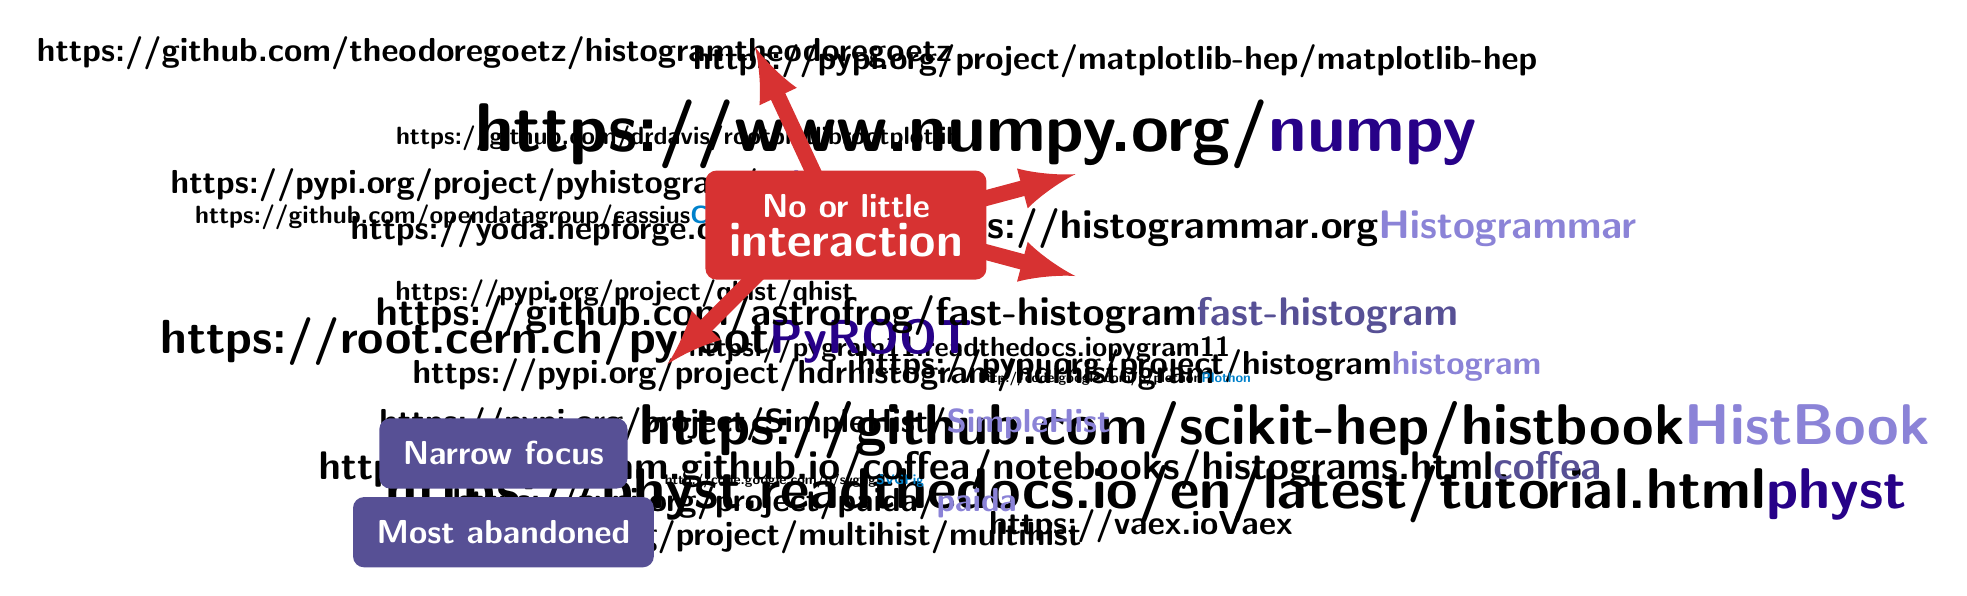
\begin{tikzpicture}[font=\sffamily\bfseries\large]
\pgfmathsetseed{40}
\node at (rand*6,rand*4)  {\huge       \href{https://github.com/scikit-hep/histbook}{\color{presLight}HistBook}};
\node at (rand*6,rand*4)  {\Large      \href{https://histogrammar.org}{\color{presLight}Histogrammar}};
\node at (rand*6,rand*4)  {\normalsize \href{https://pygram11.readthedocs.io}{pygram11}};
\node at (rand*6,rand*4)  {\small      \href{https://github.com/drdavis/rootplotlib}{rootplotlib}};
\node at (rand*6-1,rand*4){\LARGE      \href{https://root.cern.ch/pyroot}{\color{presDark}PyROOT}};
\node at (rand*6,rand*4)  {            \href{https://yoda.hepforge.org}{YODA}};
\node at (rand*6,rand*4)  {\huge       \href{https://physt.readthedocs.io/en/latest/tutorial.html}{\color{presDark}physt}};
\node at (rand*6,rand*4)  {\Large      \href{https://github.com/astrofrog/fast-histogram}{\color{presDark2}fast-histogram}};
\node at (rand*6,rand*4+.2) {\normalsize \href{https://pypi.org/project/qhist/}{qhist}};
\node at (rand*6,rand*4)  {            \href{https://vaex.io}{Vaex}};
\node at (rand*6,rand*4)  {            \href{https://pypi.org/project/hdrhistogram/}{hdrhistogram}};
\node at (rand*6,rand*4+1){            \href{https://pypi.org/project/multihist/}{multihist}};
\node at (rand*6,rand*4)  {            \href{https://pypi.org/project/matplotlib-hep/}{matplotlib-hep}};
\node at (rand*6,rand*4)  {            \href{https://pypi.org/project/pyhistogram/}{\color{presLight}pyhistogram}};
\node at (rand*6,rand*4)  {            \href{https://pypi.org/project/histogram}{\color{presLight}histogram}};
\node at (rand*6,rand*4)  {            \href{https://pypi.org/project/SimpleHist/}{\color{presLight}SimpleHist}};
\node at (rand*6,rand*4)  {            \href{https://pypi.org/project/paida/}{\color{presLight}paida}};
\node at (rand*6,rand*4)  {            \href{https://github.com/theodoregoetz/histogram}{theodoregoetz}};
\node at (2,2.25)         {\Huge       \href{https://www.numpy.org/}{\color{presDark}numpy}};
\node at (rand*6-1.5, rand*4) {\small  \href{https://github.com/opendatagroup/cassius}{\color{presLight2}Cassius}};
\node at (rand*6+3, rand*4) {\tiny     \href{http://code.google.com/p/svgfig}{\color{presLight2}SVGFig}};
\node at (rand*6, rand*4) {\tiny       \href{http://code.google.com/p/plothon}{\color{presLight2}Plothon}};
\node at (1.8, -2)        {\Large      \href{https://coffeateam.github.io/coffea/notebooks/histograms.html}{\color{presDark2}coffea}};

\node at (-4,-1.8) [white, fill=presDark2, rounded corners, inner sep=.3cm] {\large Narrow focus}; 
\node at (-4,-2.8) [white, fill=presDark2, rounded corners, inner sep=.3cm] {\large Most abandoned}; 
\begin{scope}[xshift=0.35cm, yshift=1.1cm, presHighlight]
\draw [-latex, line width=.2cm] (.5,0) -- +(15:2.5);
\draw [-latex, line width=.2cm] (-.1,0) -- +(115:2.5);
\draw [-latex, line width=.2cm] (-.5,0) -- +(225:2.5);
\draw [-latex, line width=.2cm] (.5,0) -- +(345:2.5);
\node at (0,0) [white, fill=presHighlight, rounded corners, inner sep=.3cm, align=center] {\large No or little\\ \LARGE\textbf{interaction}}; 
\end{scope}

\end{tikzpicture}
\end{document}
